%%%%%%%%%%%%%%%%%%%%%%%%%%%%%%%%%%%%%%%%%
% Short Sectioned Assignment LaTeX Template Version 1.0 (5/5/12)
% This template has been downloaded from: http://www.LaTeXTemplates.com
% Original author:  Frits Wenneker (http://www.howtotex.com)
% License: CC BY-NC-SA 3.0 (http://creativecommons.org/licenses/by-nc-sa/3.0/)
%%%%%%%%%%%%%%%%%%%%%%%%%%%%%%%%%%%%%%%%%

% \documentclass[paper=a4, fontsize=11pt]{scrartcl} % A4 paper and 11pt font size
\documentclass[11pt, a4paper]{book}
\usepackage[T1]{fontenc} % Use 8-bit encoding that has 256 glyphs
\usepackage[utf8]{inputenc}
\usepackage{fourier} % Use the Adobe Utopia font for the document - comment this line to return to the LaTeX default
\usepackage{listings} % para insertar código con formato similar al editor
\usepackage[spanish, es-tabla]{babel} % Selecciona el español para palabras introducidas automáticamente, p.ej. "septiembre" en la fecha y especifica que se use la palabra Tabla en vez de Cuadro
\usepackage{url} % ,href} %para incluir URLs e hipervínculos dentro del texto (aunque hay que instalar href)
\usepackage{graphics,graphicx, float} %para incluir imágenes y colocarlas
\usepackage[gen]{eurosym} %para incluir el símbolo del euro
\usepackage{cite} %para incluir citas del archivo <nombre>.bib
\usepackage{enumerate}
\usepackage{hyperref}
\usepackage{graphicx}
\usepackage{tabularx}
\usepackage{booktabs}
\usepackage{dirtytalk}
\usepackage{tocloft}

\usepackage[table,xcdraw]{xcolor}
\hypersetup{
	colorlinks=true,	% false: boxed links; true: colored links
	linkcolor=black,	% color of internal links
	urlcolor=cyan		% color of external links
}
\renewcommand{\familydefault}{\sfdefault}
\usepackage{fancyhdr} % Custom headers and footers
\pagestyle{fancyplain} % Makes all pages in the document conform to the custom headers and footers
\fancyhead[L]{} % Empty left header
\fancyhead[C]{} % Empty center header
\fancyhead[R]{Enrique Paubert Reca} % My name
\fancyfoot[L]{} % Empty left footer
\fancyfoot[C]{} % Empty center footer
\fancyfoot[R]{\thepage} % Page numbering for right footer
%\renewcommand{\headrulewidth}{0pt} % Remove header underlines
\renewcommand{\footrulewidth}{0pt} % Remove footer underlines
\setlength{\headheight}{13.6pt} % Customize the height of the header

\usepackage{titlesec, blindtext, color}
\definecolor{gray75}{gray}{0.75}
\newcommand{\hsp}{\hspace{20pt}}
\titleformat{\chapter}[hang]{\Huge\bfseries}{\thechapter\hsp\textcolor{gray75}{|}\hsp}{0pt}{\Huge\bfseries}
\setcounter{secnumdepth}{4}
\usepackage[Lenny]{fncychap}

% Creación de la lista de definiciones
\newcommand{\listDefname}{Índice de definiciones}
\newlistof{Def}{def}{\listDefname}
\newcommand{\Def}[1]{
\refstepcounter{Def}
\textbf{#1\label{Def:#1}}
\addcontentsline{def}{Def}
{\protect\numberline{\theDef}#1}}
% \Def{ejemplo} -> Declarar una definición
% \ref{Def:ejemplo} -> Referenciar una definición

\begin{document}

% Plantilla portada UGR
\begin{titlepage}
\newlength{\centeroffset}
\setlength{\centeroffset}{-0.5\oddsidemargin}
\addtolength{\centeroffset}{0.5\evensidemargin}
\thispagestyle{empty}

\noindent\hspace*{\centeroffset}\begin{minipage}{\textwidth}

\centering

\includegraphics[width=0.9\textwidth]{logos/logo_ugr.jpg}\\[1.4cm]

\textsc{ \Large TRABAJO FIN DE GRADO\\[0.2cm]}
\textsc{ GRADO EN INGENIERIA INFORMATICA}\\[1cm]

{\Huge\bfseries Título \\}
\noindent\rule[-1ex]{\textwidth}{3pt}\\[3.5ex]
{\large\bfseries Subtítulo }
\end{minipage}

\vspace{2.5cm}
\noindent\hspace*{\centeroffset}
\begin{minipage}{\textwidth}
\centering

\textbf{Autor}\\ {Estudiante}\\[2.5ex]
\textbf{Director}\\ {Tutor(a)(es)}\\[2cm]

\includegraphics[width=0.3\textwidth]{logos/etsiit_logo.png}\\[0.1cm]
\textsc{Escuela Técnica Superior de Ingenierías Informática y de Telecomunicación}\\
\textsc{---}\\
Granada, Junio de 201x
\end{minipage}
\end{titlepage}


% Plantilla prefacio UGR
\thispagestyle{empty}

\begin{center}
{\large\bfseries Port de un sistema operativo de tiempo real a una placa ARM \\ FreeRTOS en ARM7TDMI-S }\\
\end{center}
\begin{center}
Enrique Paubert Reca\\
\end{center}

%\vspace{0.7cm}

\vspace{0.5cm}
\noindent\textbf{Palabras clave}: \textit{software libre}, \textit{sistema operativo de tiempo real}, \textit{RTOS}, \textit{tiempo real}, \textit{ARM}, \textit{sistemas embebidos}
\vspace{0.7cm}

\noindent\textbf{Resumen}\\
	

\cleardoublepage

\begin{center}
	{\large\bfseries Same, but in English}\\
\end{center}
\begin{center}
	Enrique Paubert Reca\\
\end{center}
\vspace{0.5cm}
\noindent\textbf{Keywords}: \textit{open source}, \textit{floss}
\vspace{0.7cm}

\noindent\textbf{Abstract}\\


\cleardoublepage

\thispagestyle{empty}

\noindent\rule[-1ex]{\textwidth}{2pt}\\[4.5ex]

D. \textbf{Tutora/e(s)}, Profesor(a) del ...

\vspace{0.5cm}

\textbf{Informo:}

\vspace{0.5cm}

Que el presente trabajo, titulado \textit{\textbf{Port de un sistema operativo de tiempo real a una placa ARM}},
ha sido realizado bajo mi supervisión por \textbf{Enrique Paubert Reca}, y autorizo la defensa de dicho trabajo ante el tribunal
que corresponda.

\vspace{0.5cm}

Y para que conste, expiden y firman el presente informe en Granada a Junio de 2024.

\vspace{1cm}

\textbf{El/la director(a)/es: }

\vspace{5cm}

\noindent \textbf{(nombre completo tutor/a/es)}

\chapter*{Agradecimientos}

A mis padres, por estar ahí a pesar de todo lo que ha costado.

A Juan Pedro, porque sin el no habría empezado esta carrera.

A Shei, porque sin ella no la habría terminado.






% Índice de contenidos
\newpage
\tableofcontents

% Índice de imágenes y tablas
\newpage
% Índice de definiciones
\listofDef

% lista de imágenes
\listoffigures

% Si hay suficientes se incluirá dicho índice
\listoftables
\newpage

% Introducción 
\chapter{Introducción}

Este proyecto es software libre, y está liberado con la licencia \cite{gplv3}.

\section{Motivación}

La motivación de este Trabajo de Fin de Grado surgió tras cursar la asignatura de Sistemas Empotrados del grado. Sentí que, aunque habíamos trabajado muy bien la base de los sistemas con el mismo nombre, quería profundizar algo más porque es un tema que considero muy interesante. 

Además, durante los años de la carrera, había oído hablar de los sistemas operativos de tiempo real, que también llamaron mucho mi atención, de manera que he decidido trabajar estos dos intereses en este proyecto.  



Tras cursar la asignatura de Sistemas Empotrados sentí que quería profundizar en mi conocimiento de estos sistemas en mi trabajo de fin de grado. Además, durante el grado había oido hablar de sistemas de tiempo real, pero no había trabajado con ninguno. De manera que he juntado estos dos intereses en este proyecto.


\section{Estructura}
\begin{enumerate}
    \item \textbf{Introducción:} En este capítulo se aborda la motivación del proyecto y se describe la estructura del documento.
    \item \textbf{Descripción del problema:} Se detallan el objetivo del proyecto, las restricciones a considerar y los requisitos necesarios para llevarlo a cabo.
    \item \textbf{Antecedentes:} Se presenta el contexto tecnológico, definiciones y datos relevantes que permiten comprender el entorno de los sistemas empotrados y de tiempo real.
    \item \textbf{Estudio de requisitos:} En este apartado se describen los casos de uso, los requisitos y los actores que definen y limitan el alcance del proyecto.
    \item \textbf{Análisis del problema:} Se analizan las decisiones relacionadas con la elección de hardware y software para asegurar el correcto funcionamiento del sistema.
    \item \textbf{Planificación:} Se establece un cronograma para el proyecto y se discuten otros factores importantes como el presupuesto y las fases de implementación del mismo.
    \item \textbf{Implementación:} Se detalla el proceso de implementación del proyecto, siguiendo las fases definidas en la planificación y abordando los problemas encontrados en las diferentes etapas.
    \item \textbf{Conclusiones y trabajos futuros:} Este capítulo final ofrece una valoración del trabajo realizado, detalla los conocimientos adquiridos durante la realización de este proyecto y propone posibles líneas de trabajo futuras.
\end{enumerate}


% Descripción del problema y hasta donde se llega
\chapter{Descripción del problema}
\section{El problema}
En la actualidad existen multitud de placas diseñadas para sistemas embebidos, así como una gran cantidad de sistemas operativos y firmwares que se utilizan para facilitar el desarrollo de aplicaciones para las mismas.
Para muchas de estas aplicaciones modernas es útil o necesario el uso de sistemas de tiempo real, pues permite establecer restricciones de tiempo predecibles y consistentes, además de poder crear una planificación que se ajuste a nuestros objetivos.\\
El problema radica en la inmensa cantidad de placas que, aun teniendo los requisitos necesarios para el proyecto que tengamos entre manos, carecen de la posibilidad de utilizar un RTOS, perdiendo flexibilidad y aumentando los tiempos de desarrollo, y obligándonos a buscar opciones que no sean tan favorables.
Además los sistemas operativos de tiempo real prediminantemente utilizados en la industria son desarrollados por empresas que poseen software propietario, lo que dificulta el aprendizaje y el acceso a estos sistemas.

% En la actualidad, el uso de sistemas embebidos esta creciendo de manera exponencial en nuestra sociedad, así como la implementación de sistemas operativos de tiempo real (RTOS). Si bien estos últimos estan implementados en multitud de placas de sistemas empotrados, aún existe un gran número de placas que no tienen posibilidad de utilizar este RTOS, perdiendo la flexibilidad y la funcionalidad que estos podrian ofrecer.

\section{La solución}
Se propone la realización de una adaptación o \textit{port} de un sistema operativo de tiempo real a una placa ARM con el objetivo de aprender sobre la arquitectura de los sistemas operativos, las restricciones de el tiempo real 

% \itemize


% Estado del arte
% 	1. Crítica al estado del arte
% 	2. Propuesta
\chapter{Antecedentes}

\noindent\fbox{
	\parbox{\textwidth}{
    En este capítulo hablaré de el contexto actual en el que se desarrolla este projecto y daré algunas definiciones relevantes.
	}
}\\

El software libre y sus licencias \cite{gplv3} ha permitido llevar a cabo una expansión del aprendizaje de la informática sin precedentes.

\section{Descripción de la tecnología}
\subsection{Sistemas embebidos}
% NOTE: "ordenadores" o "sistemas informáticos"?
Cuando hablamos de ordenadores generalmente se piensa sobremesas o portátiles, y tal vez en teléfonos inteligentes, tablets o tal vez incluso servidores. A pesar de la ubicuidad de estos sistemas, muchos de los ordenadores con los que interactuamos a diario son invisibles, estan embebidos.

% \begin{center}\colorbox{cyan!10}{\fbox{ \begin{minipage}{11cm}
Los \Def{Sistemas Embebidos} son combinaiones de software y hardware (opcionalmente con partes mecánicas), de proposito específico y con un número reducido y definido de funciones. Pueden ser independientes o formar parte de otro sistema. Generalmente tienen una serie de restricciones como el uso de energía y capacidad para trabajar bajo condiciones adversas. Ejemplos: Lector de tarjetas de metro o autobús, TV, router, frigorífico, TPV, la multitud de sistemas que hay en un coche... \cite{es_glossary} \cite{marwedel}
% \end{minipage} }} \end{center}

% \begin{center}\colorbox{cyan!10}{\fbox{ \begin{minipage}{11cm}
En cambio, los \textbf{ordenadores de propósito general} es una combinación de hardware y software diseñados para un proposito general, es decir, sin un límite establecido de funiciones. Ejemplos: PC, teléfono inteligente, servidor... \cite{es_glossary}
% \end{minipage} }} \end{center}

Dos ejemplos claros de la diferencia entre un sistema empotrado y uno de proposito general serían la Nintendo Switch y la Steam Deck. La Nintendo Switch es un sistema empotrado, una consola diseñada para jugar a videojuegos que no tiene, por ejemplo, la función de navegar por internet por motivos de seguridad. La Steam Deck es un sistema con un factor de forma similar pero es un ordenador de proposito general que no ha sido limitado por diseño, aunque su principal proposito sea el de jugar a videojuegos.

% TODO: Insertar imágenes de Switch y Steam Deck aqui
%
%
%
%
%

\begin{center} \colorbox{yellow!10} { \fbox{ \begin{minipage}{11cm}
				Existe un debate sobre si teléfono o una tablet es un sistema empotrado, y con respecto a los \textit{dumbphones} o móviles no inteligentes es cierto dado que tienen un reducido número de funciones, pero mi opinión es que los móviles actuales se pueden utilizar como ordenadores de propósito general y la línea entre tablet y portátil se difumina cada vez más.
			\end{minipage} } } \end{center}

\subsubsection{BSPs}
Un \Def{Board Support Package} o BSP en el contexto de los sistemas empotrados es un \textit{firmware} diseñado para un hardware concreto que proporciona una secuencia de arranque y drivers para los dispositivos de la placa, entre otras funciones.

\subsection{RISC}
\Def{RISC}

\subsection{ARM}
\Def{ARM}

\subsection{Computación en Tiempo Real}
Los sistemas de \Def{Tiempo Real} son un tipo de sistema donde el funcionamiento correcto del mismo no depende solamente de que el resultado lógico sea correcto, sino también del tiempo requerido para llegar a ese resultado \cite{stankovic}. Esto no quiere decir necesariamente que las tareas deban tardar el mínimo tiempo posible, sino que el tiempo que se tarda en realizar una tarea debe de ser acotado, predecible y consistente.

Un ejemplo de como la consistencia se valora más que la velocidad es que en muchos sistemas de tiempo real no se utiliza memoria caché, ya que a pesar de que puede acelerar la computación, los aciertos y fallos de caché son difíciles de predecir y pueden provocar inconsistencias en el tiempo de ejecución \cite{MILLIGAN1996}.

La computación en tiempo real puede aplicarse tanto a ordenadores como sistemas empotrados y redes de comunicaciones. Algunos ejemplos incluyen sistemas de control de procesos, sistemas de conducción autónoma y sistemas de control de tráfico aéreo.

\subsubsection{Tiempo real «duro» y «blando»}
Cuando hablamos de sistemas de tiempo real existe la distinción entre sistemas de tiempo real «duros» (\textit{hard real time}) y «blandos» (\textit{soft real time}). \textit{Hard real time} se refiere a sistemas críticos donde una \textit{deadline} no cumplida puede tener resultados catastróficos, como puede ser en campos como la medicina o la aeroespacial. En cambio el \textit{soft real time} abarca problemas donde las \textit{deadline} no son tan estrictas y incumplirlas degradará la experiencia pero el sistema podrá seguir funcionando. Ejemplos de esto son el \textit{streaming} de elementos multimedia o la comunicación utilizando \textit{VoIP (Voice over IP)}. Mientras que el tiempo real «blando» se suele implementar dentro de otros sistemas que no requieren tiempo real, el tiempo real «duro» se implementa dentro de sistemas especialiados.

Dos ejemplos que muestran esta distinción son el ABS de un coche y una videoconsola. El ABS es un sistema de tiempo real «duro» ya que si no reacciona a tiempo puede provocar una colisión. En cambio una videoconsola es un sistema de tiempo real blando, debe realizar los cálculos necesarios para cada \textit{frame} del juego a tiempo de manera que se mantenga un \textit{framerate} estable, pero si se retrasa alguno se puede seguir jugando al juego.\\

Esta clasificación de «duro» y «blando» es más un espectro. Hay sistemas con mayores y menores tolerancias pero no existe una linea definida que separe claramente los sistemas de tiempo real «duros» y «blandos». Aun así la mayoría del trabajo de investigación que se realiza entorno al tiempo real se refiere a la parte del espectro que se considera tiempo real «duro».

También en este espectro existen el \textit{firm real time} que se refiere a sistemas donde, si no se alcanza una \textit{deadline}, el resultado de la operacion es irrelevante. Un ejemplo es un sistema que predice el tiempo, si el cálculo de la simulación es que va a llover pero ya ha empezado a llover el resultado no sirve para nada \cite{wang2017rtes}.

\subsubsection{Sistemas Operativos de Tiempo Real}
Los sistemas de tiempo real «duro» suelen utilizar sistemas operativos especializados llamados \Def{Sistemas operativos de tiempo real} (\textit{RTOS} por sus siglas en inglés). La diferencia más importante de los sistemas operativos de tiempo real con respecto a los de propósito general es la planificación. estos últimos utilizan \textit{FIFO}, \textit{Round-Robin} o colas con prioridad entre otros (o una combinación de varios) para planificar las tareas que el sistema o los usuarios van creando y terminando.

Los sistemas de tiempo real tienen una filosofia muy distinta, ya que el sistema va a tener un número muy reducido de funciones y tareas en comparación a un sistema operativo tradicional, pero también cada tarea tendrá un tiempo límite en el que debe completarse o \textit{deadline}. Por ello, la planificación debe calcularse en el peor caso (con el máximo número de tareas que se dará en la realidad), ya sea manualmente o con un algoritmo, para que todas las tareas terminen dentro de su \textit{deadline}.

Algunos de los sitemas operativos de tiempo real más utilizados son Deos, embOS, FreeRTOS, Integrity y Keil RTX \cite{lynx2024rtos}.

\subsection{Importancia del tiempo real en sistemas embebidos}
% TODO:
\textbf{\textcolor{cyan}{TODO: no se si hacer esta sección}} 

Muchos de los sistemas de tiempo real duro son implementados como sistemas embebidos\\

Ejemplos...

% A Closer Look In the fast-paced world of technology, embedded systems have become ubiquitous, powering devices that range from the everyday to the extraordinary. Real-Time Operating Systems (RTOS) are the unsung heroes that ensure these embedded systems meet the precise and time-sensitive demands of their applications. Let’s delve deeper into the significance of RTOS, exploring specific applications, key components, and emerging trends in the realm of embedded systems.
%
% # Applications
% Automotive Systems
% Medical Devices
% Industrial Automation
% Telecommunications
%
% # Where RTOS within embedded is mostly used? 
% In the automotive industry, RTOS finds extensive use across a range of applications, especially for FuSa compliance
% In the aerospace and aviation sector, RTOS is essential for real-time decision-making in various applications. 
% In the field of medical devices, RTOS is fundamental to the operation of key devices.
% RTOS is widely utilized in the domain of industrial automation, primarily for applications that require real-time control and monitoring
% In industries like consumer electronics, RTOS finds widespread applications.
%
% # Why use RTOS
% Maintainability/Extensibility
% Modularity
% Improved efficiency?
% Easier control over peripherals -> provide a good mutual exclusion mechanism. 
%
% # Links
% Real-time operating systems are the only practical solution for use in embedded systems, especially in scenarios were multiple control loops are required to behave predictably under controlled priority levels.
% https://iies.in/blog/what-is-the-role-of-rtos-in-embedded-systems/
% https://www.freertos.org/FAQWhat.html#WhyUseRTOS
% https://moschip.com/blog/semiconductor/real-time-operating-systems-rtos-in-embedded-systems/
% https://www.intervalzero.com/the-role-of-an-rtos-in-an-embedded-system/


\section{Breve Historia}
\textbf{\textcolor{red}{Tal vez no debería de hacer esta sección}} 

% NOPE:
% NOTE:VALE vamos a hacer esto distinto. Una timeline desde los 40-50 hasta el presente y pongo hitos relevantes tanto para tiempo real como sistemas empotrados. Un color para SE, un color para RT y otro para cosas de computación en general.

\subsection{Tiempo real}
\subsection{Sistemas embebidos}

% FIXME: Voy a acabar borrando todo esto, no es relevante
% \subsubsection{Breve historia de los microprocesadores}
% \begin{itemize}
% 	\item (1950-1960) Primeros Circuitos integrados
% 	      \begin{itemize}
% 		      \item Invención de los circuitos integrados híbridos (Jack Kilby) y monolíticos (Robert Noyce).
% 	      \end{itemize}
% 	\item (1970-1980) Grandes avances en microprocesadores siguiendo la ley de Moore.
% 	      \begin{itemize}
% 		      \item Intel 4004, 8008, 8086...
% 		      \item Apple 1
% 		      \item Z80
% 		      \item Motorola 68000
% 	      \end{itemize}
% 	\item (1990-2000) Sistemas embebidos en productos comerciales
% 	      \begin{itemize}
% 		      \item Arquitectura ARM6
% 		      \item Java: Compilar una vez, ejecutar en multitud de dispositivos.
% 	      \end{itemize}
% 	\item (2010-presente) Acceso a microprocesadores facilitado por:
% 	      \begin{itemize}
% 		      \item Rasperry Pi
% 		      \item Arduino
% 		      \item IoT
% 	      \end{itemize}
% \end{itemize}

Los primeros ordenadores eran mainframes sin sistema operativo y con un número reducido de funciones, por lo que tenían más en común con un sistema empotrado que con un ordenador de propósito general moderno. Aun así esa diferenciación ocurriría hasta más tarde.

El Computador de Navegación del Apollo (AGC por sus siglas en inglés) se considera uno de los primeros sistemas embebidos de la historia. Fue utilizado en las misiones Apollo para controlar la orientación y navegación de los módulos de mando y lunares.

\section{Aplicaciones}




\chapter{Estudio de requisitos}

\section{Actores}

El producto final de este proyecto es un port que en el futuro un desarrollador utilizará para crear un proyecto. Por tanto, en el análisis de requisitos, este futuro desarrollador es el principal y único actor. \autoref{AC-01}.

\begin{table}[!ht]
    \begin{tabular}{|llllll|}
	\hline
	\multicolumn{1}{|l|}{\textbf{Actor}}		& \multicolumn{4}{l|}{Desarrollador}	& AC-01	    \\ \hline
	\multicolumn{1}{|l|}{\textbf{Descripción}}     	& \multicolumn{5}{l|}{Persona que utiliza el port para hacer un proyecto con la placa}	    \\ \hline
	% \multicolumn{1}{|l|}{\textbf{Características}}	& \multicolumn{5}{l|}{Programar}	\\ \hline
	% \multicolumn{1}{|l|}{\textbf{Relaciones}}		& \multicolumn{5}{l|}{Diseña tareas que luego FreeRTOS ejecuta}	    \\ \hline
	\multicolumn{1}{|l|}{\textbf{Referencias}}     	& \multicolumn{5}{l|}{RF0, RF1}	\\ \hline
	\multicolumn{1}{|l|}{\textbf{Autor}}           	& \multicolumn{1}{l|}{Enrique Paubert}        & \multicolumn{1}{l|}{\textbf{Fecha}}        & \multicolumn{1}{l|}{10/08/2024}        & \multicolumn{1}{l|}{\textbf{Versión}}       & 1.0                   \\ \hline
	% \multicolumn{6}{|l|}{\textbf{\underline{Atributos}}} \\ \hline % \cellcolor[HTML]{DAE8FC}
	% \multicolumn{1}{|l|}{\textbf{Nombre}}		& \multicolumn{4}{l|}{\textbf{Descripción}} &  \textbf{Tipo}  \\ \hline
	% \multicolumn{1}{|l|}{ - }				& \multicolumn{4}{l|}{ - }  &  -      \\ \hline
    \end{tabular}
    \caption[Actor: Desarrollador]{Especificación del actor Desarrollador.}
    \label{AC-01}
\end{table}

\section{Casos de Uso}

Los casos de uso recogerán las interacciones que puede tener el futuro desarrollador con el port. Tablas \ref{CU-01}, \ref{CU-02}, \ref{CU-03} y \ref{CU-04}.

\begin{table}[!ht]
    \begin{tabular}{|l|l|l|l|l|l|}
	\hline
	\textbf{Caso de Uso} & \multicolumn{3}{l|}{Configurar el sistema} & \multicolumn{2}{l|}{CU-01} \\ \hline
	\textbf{Actores} & \multicolumn{5}{l|}{Desarrollador} \\ \hline
	\textbf{Tipo} & \multicolumn{5}{l|}{Primario, Esencial} \\ \hline
	\textbf{Referencias} & RF0 & \multicolumn{4}{l|}{-} \\ \hline
	\textbf{Precondición} & \multicolumn{5}{l|}{El sistema tiene una configuración concreta} \\ \hline
	\textbf{Postcondición} & \multicolumn{5}{l|}{La configuración del sistema ha cambiado} \\ \hline
	\textbf{Autor} & Enrique Paubert & \textbf{Fecha} & 10/08/2024 & \textbf{Versión} & 1.0 \\ \hline
	% \multicolumn{6}{|l|}{\textbf{\underline{Propósito}}} \\ \hline %\cellcolor[HTML]{ECF4FF}
	% \multicolumn{6}{|l|}{Que el desarrollador pueda configurar el sistema según sus necesidades} \\ \hline
	% \multicolumn{6}{|l|}{\textbf{\underline{Resumen}}} \\ \hline % \cellcolor[HTML]{ECF4FF}
	% \multicolumn{6}{|l|}{\begin{tabular}[c]{@{}l@{}}1. El desarollador configura el sistema.\\  2. -. \\ 3. profit.\end{tabular}} \\ \hline
    \end{tabular}%
    \caption{Caso de uso de configurar el sistema}
    \label{CU-01}
\end{table}

\begin{table}[!ht]
    \begin{tabular}{|l|l|l|l|l|l|}
	\hline
	\textbf{Caso de Uso} & \multicolumn{3}{l|}{Diseñar una tarea} & \multicolumn{2}{l|}{CU-02} \\ \hline
	\textbf{Actores} & \multicolumn{5}{l|}{Desarrollador} \\ \hline
	\textbf{Tipo} & \multicolumn{5}{l|}{Primario, Esencial} \\ \hline
	\textbf{Referencias} & RF1 & \multicolumn{4}{l|}{-} \\ \hline
	\textbf{Precondición} & \multicolumn{5}{l|}{-} \\ \hline
	\textbf{Postcondición} & \multicolumn{5}{l|}{Existe una función que puede actuar como tarea} \\ \hline
	\textbf{Autor} & Enrique Paubert & \textbf{Fecha} & 10/08/2024 & \textbf{Versión} & 1.0 \\ \hline
	% \multicolumn{6}{|l|}{\textbf{\underline{Propósito}}} \\ \hline %\cellcolor[HTML]{ECF4FF}
	% \multicolumn{6}{|l|}{El desarrollador diseña una tarea} \\ \hline
	% \multicolumn{6}{|l|}{\textbf{\underline{Resumen}}} \\ \hline % \cellcolor[HTML]{ECF4FF}
	% \multicolumn{6}{|l|}{\begin{tabular}[c]{@{}l@{}}1. El desarollador crea una tarea.\\  2. -. \\ 3. profit.\end{tabular}} \\ \hline
    \end{tabular}%
    \caption{Caso de uso de diseñar una tarea}
    \label{CU-02}
\end{table}

\begin{table}[!ht]
    \begin{tabular}{|l|l|l|l|l|l|}
	\hline
	\textbf{Caso de Uso} & \multicolumn{3}{l|}{Crear una instancia de una tarea} & \multicolumn{2}{l|}{CU-03} \\ \hline
	\textbf{Actores} & \multicolumn{5}{l|}{Desarrollador} \\ \hline
	\textbf{Tipo} & \multicolumn{5}{l|}{Primario, Esencial} \\ \hline
	\textbf{Referencias} & RF1 & \multicolumn{4}{l|}{-} \\ \hline
	\textbf{Precondición} & \multicolumn{5}{l|}{Existe una función que puede actuar como tarea} \\ \hline
	\textbf{Postcondición} & \multicolumn{5}{l|}{Se añadirá una instancia de esta tarea al sistema} \\ \hline
	\textbf{Autor} & Enrique Paubert & \textbf{Fecha} & 10/08/2024 & \textbf{Versión} & 1.0 \\ \hline
	% \multicolumn{6}{|l|}{\textbf{\underline{Propósito}}} \\ \hline %\cellcolor[HTML]{ECF4FF}
	% \multicolumn{6}{|l|}{???} \\ \hline
	% \multicolumn{6}{|l|}{\textbf{\underline{Resumen}}} \\ \hline % \cellcolor[HTML]{ECF4FF}
	% \multicolumn{6}{|l|}{\begin{tabular}[c]{@{}l@{}}1. El desarollador crea una tarea.\\  2. -. \\ 3. profit.\end{tabular}} \\ \hline
    \end{tabular}%
    \caption{Caso de uso de crear una instancia de una tarea}
    \label{CU-03}
\end{table}

\begin{table}[!ht]
    \begin{tabular}{|l|l|l|l|l|l|}
	\hline
	\textbf{Caso de Uso} & \multicolumn{3}{l|}{Eliminar una instancia de una tarea} & \multicolumn{2}{l|}{CU-04} \\ \hline
	\textbf{Actores} & \multicolumn{5}{l|}{Desarrollador} \\ \hline
	\textbf{Tipo} & \multicolumn{5}{l|}{Primario, Esencial} \\ \hline
	\textbf{Referencias} & RF1 & \multicolumn{4}{l|}{-} \\ \hline
	\textbf{Precondición} & \multicolumn{5}{l|}{Hay una instancia de una tarea en el sistema} \\ \hline
	\textbf{Postcondición} & \multicolumn{5}{l|}{Se elimina dicha instancia de la tarea del sistema} \\ \hline
	\textbf{Autor} & Enrique Paubert & \textbf{Fecha} & 10/08/2024 & \textbf{Versión} & 1.0 \\ \hline
	% \multicolumn{6}{|l|}{\textbf{\underline{Propósito}}} \\ \hline %\cellcolor[HTML]{ECF4FF}
	% \multicolumn{6}{|l|}{???} \\ \hline
	% \multicolumn{6}{|l|}{\textbf{\underline{Resumen}}} \\ \hline % \cellcolor[HTML]{ECF4FF}
	% \multicolumn{6}{|l|}{\begin{tabular}[c]{@{}l@{}}1. El desarollador crea una tarea.\\  2. -. \\ 3. profit.\end{tabular}} \\ \hline
    \end{tabular}%
    \caption{Caso de uso de eliminar una instancia de una tarea}
    \label{CU-04}
\end{table}

\section{Diagramas de casos de uso}
En este diagrama mostraré cómo el desarrollador interacciona con el sistema. \autoref{fig:UML}.

\begin{figure}[!ht]
\centering
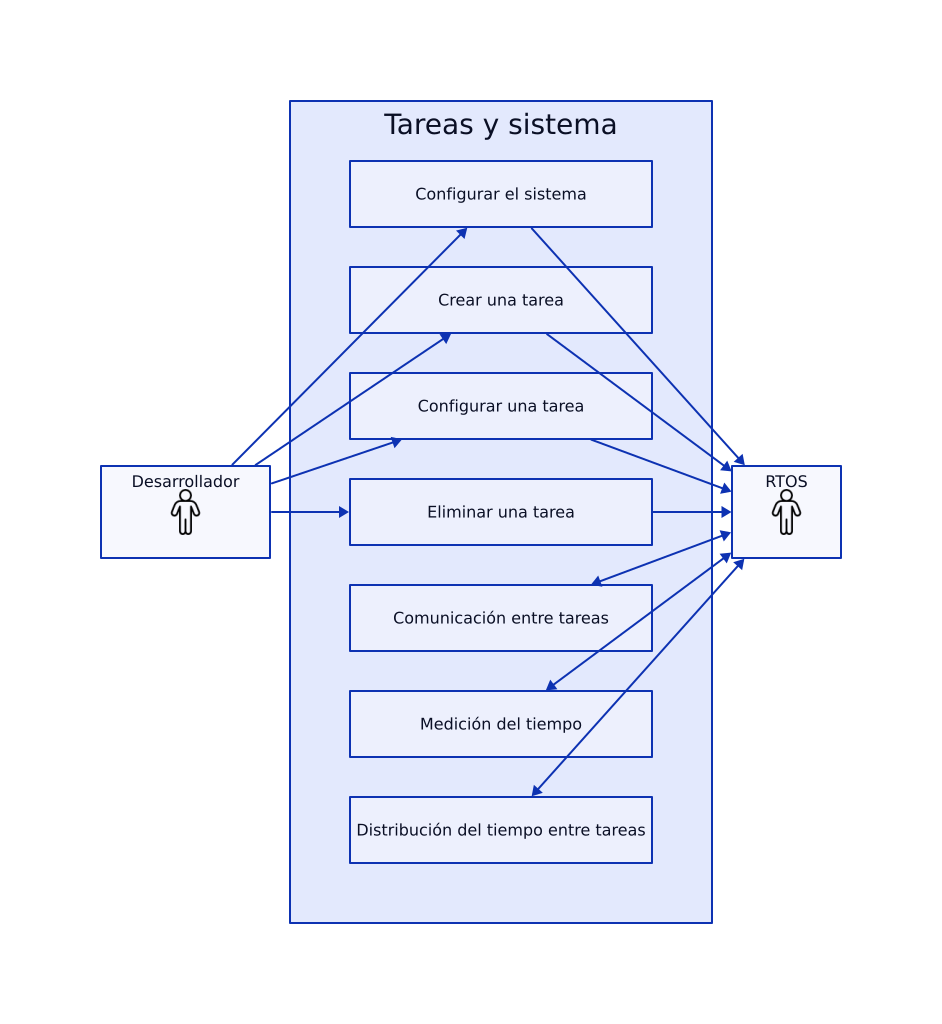
\includegraphics[width=\textwidth]{img/UML1.png}
\caption{Diagrama UML de las tareas}
\label{fig:UML}
\end{figure}

\section{Requisitos}
Los requisitos funcionales describen especifican qué debe de hacer el sistema, mientras que los no funcionales describen cómo debe de hacerlo.

\subsection{Requisitos no funcionales}
Empezaremos listando los requisitos no funcionales ya que imponen ciertas restricciones esenciales que afectan al diseño del sistema.

% \subsubsection{Uso obligatorio de FreeRTOS:}
% El sistema debe usar FreeRTOS como el sistema operativo en tiempo real (RTOS). Este proyecto fue concebido en un principio para utilizar FreeRTOS.
%
% \subsubsection{Uso obligatorio de la Redwire Econotag R3:}
% El port debe estar diseñado para funcionar en la placa Redwire Econotag R3. Esta placa es la utilizada en la asignatura de sistema empotrados. Dado que este proyecto se plantea como una profundización en esta asignatura, tiene sentido utilizar la misma placa.
%
% \subsubsection{Uso del BSP desarrollado en SE:}
% Se debe utilizar un BSP desarrollado en una asignatura de sistemas empotrados. Al igual que en el requisito anterior, se debe a que este proyecto es una expansión de esa asignatura.
%
% \subsubsection{Eficiencia del sistema:}
% El sistema debe ser eficiente en cuanto a consumo de recursos, minimizando el uso de CPU y memoria. Dado que se trata de un sistema embebido con recursos limitados, es crucial optimizar el uso de los mismos.
%
% \subsubsection{Documentación y mantenibilidad:}
% El código y la configuración del sistema deben estar bien documentados para facilitar su mantenimiento y posibles futuras modificaciones. La calidad de la documentación es crucial para el mantenimiento a largo plazo y para la colaboración con otros desarrolladores.
%

\begin{itemize}
    \item \textbf{RNF-01 - Uso obligatorio de FreeRTOS:} El sistema debe usar FreeRTOS como el sistema operativo en tiempo real (RTOS). Este proyecto fue concebido en un principio para utilizar FreeRTOS.
    \item \textbf{RNF-02 - Uso obligatorio de la Redwire Econotag R3:} El port debe estar diseñado para funcionar en la placa Redwire Econotag R3. Esta placa es la utilizada en la asignatura de sistema empotrados. Dado que este proyecto se plantea como una profundización en esta asignatura, tiene sentido utilizar la misma placa.
    \item \textbf{RNF-03 - Uso del BSP desarrollado en SE:} Se debe utilizar un BSP desarrollado en una asignatura de sistemas empotrados. Al igual que en el requisito anterior, se debe a que este proyecto es una expansión de esa asignatura.
    \item \textbf{RNF-04 - Eficiencia del sistema:} El sistema debe ser eficiente en cuanto a consumo de recursos, minimizando el uso de CPU y memoria. Dado que se trata de un sistema embebido con recursos limitados, es crucial optimizar el uso de los mismos.
    \item \textbf{RNF-05 - Documentación y mantenibilidad:} El código y la configuración del sistema deben estar bien documentados para facilitar su mantenimiento y posibles futuras modificaciones. La calidad de la documentación es crucial para el mantenimiento a largo plazo y para la colaboración con otros desarrolladores.
\end{itemize}

\subsection{Requisitos funcionales}

% \subsubsection{Tiempo real}
% El port debe de garantizar que el sistema funcione con restricciones de tiempo real.
%
% \subsubsection{Gestión de tareas:}
% El sistema debe permitir la correcta creación, gestión y eliminación de tareas.
%
% \subsubsection{Soporte para periféricos:}
% El port debe incluir, mediante el BSP, soporte para los periféricos principales de la Econotag, (GPIO, UART...).
%
% \subsubsection{Configuración del Sistema}
% El sistema debe permitir la configuración de parámetros de FreeRTOS, como tamaño de RAM asignada tanto al sistema operativo como a las tareas, frecuencia del tick del sistema, y configuración de prioridades, adaptándose a las necesidades de las aplicaciones que se quieran desarrollar en el futuro.
%
% \subsubsection{Demo y validación}
% Se incluirá una demo que demuestre el correcto funcionamiento del sistema.

\begin{itemize}
    \item \textbf{RF-01 - Tiempo real:} El port debe de garantizar que el sistema funcione con restricciones de tiempo real.
    \item \textbf{RF-02 - Gestión de tareas:} El sistema debe permitir la correcta creación, gestión y eliminación de tareas.
    \item \textbf{RF-03 - Soporte para periféricos:} El port debe incluir, mediante el BSP, soporte para los periféricos principales de la Econotag, (GPIO, UART...).
    \item \textbf{RF-04 - Configuración del Sistema:} El sistema debe permitir la configuración de parámetros de FreeRTOS, como tamaño de RAM asignada tanto al sistema operativo como a las tareas, frecuencia del \emph{tick} del sistema, y configuración de prioridades, adaptándose a las necesidades de las aplicaciones que se quieran desarrollar en el futuro.
    \item \textbf{RF-05 - Demo y validación:} Se incluirá una demo que demuestre el correcto funcionamiento del sistema.
\end{itemize}


\chapter{Planificación}

\section{Etapas}

Voy a dividir la planificación en tres etapas, aprendizaje, desarrollo y depuración. Cada una de estas fases contendrán pasos que he seguido en la implementación asociados a ellos.

\subsection{Etapa 1: Aprendizaje}
La primera fase consiste en la recopilación de información y el aprendizaje necesario para realizar el proyecto.

\begin{itemize}
\item Familiarizarse con la estructura de FreeRTOS
\item (Re)familiarizarse con el BSP
\end{itemize}

\subsection{Etapa 2: Desarrollo}
\begin{itemize}
\item Creación de los archivos necesarios para el port
\item Integración del BSP
\item Preparación de los CMakeFiles y primera compilación
\item Ampliación del BSP
\item Modificación de los archivos del port
\end{itemize}

\subsection{Etapa 3: Depuración}
\begin{itemize}
\item Demo básica
\item Demo ampliada
\end{itemize}

\section{Temporización}
Esta temporización supone una semana de trabajo de 20 horas. De media se realizarán cuatro horas de trabajo al día cinco días a la semana.

\begin{table}[h!]
\centering
\begin{tabularx}{\textwidth}{|X|c|c|c|}
\hline
\textbf{Tarea} & \textbf{Tiempo estimado} & \textbf{Fecha inicio} & \textbf{Fecha fin} \\ \hline
Familiarizarse con la estructura de FreeRTOS & 1 semana & 15/05/2024 & 21/05/2024 \\ \hline
(Re)familiarizarse con el BSP & 1 semana & 29/05/2024 & 04/06/2024 \\ \hline
Creación de los archivos necesarios para el port & 1 semana & 22/05/2024 & 28/05/2024 \\ \hline
Integración del BSP & 1.5 semanas & 05/06/2024 & 14/06/2024 \\ \hline
Preparación de los CMakeFiles y primera compilación & 1.5 semanas & 17/06/2024 & 26/06/2024 \\ \hline
Ampliación del BSP & 1.5 semanas & 27/06/2024 & 08/07/2024 \\ \hline
Modificación de los archivos del port & 1 semana & 09/07/2024 & 15/07/2024 \\ \hline
Demo básica & 1 semana & 16/07/2024 & 22/07/2024 \\ \hline
Demo ampliada & 1.5 semanas & 23/07/2024 & 1/08/2024 \\ \hline
\end{tabularx}
\caption{Plan de trabajo para el proyecto.}
\label{tabla:plan_trabajo}
\end{table}

\begin{figure}[!ht]
\centering
\includegraphics[width=\textheight, angle=270]{img/Temporización-TFG.png}
\caption{Diagrama de Gantt de la temporización}
\label{fig:Gantt_1}
\end{figure}

\section{Presupuesto}
\emph{WITTENSTEIN High Integrity Systems} ofrece como servicio la realización de un port de FreeRTOS a una plataforma que no lo soporte, así que contacté con ellos para saber cual sería el presupuesto de un proyecto similar a este pero no recibí respuesta.

\subsection{Sueldo}
Según lo comentado por mi tutor y lo observado en diversas ofertas de trabajo por Internet, el sueldo usual de un ingeniero de sistemas embebidos \emph{junior} ronda los 20.000€ al año. Convertido a salario por hora, esto son 9.62€/hora. La duración prevista del proyecto son una 11 semanas, trabajando 20 horas semanales. $11 * 20 = 220$ horas totales. La remuneración total sería $220 * 9,62 = 2116,40$€.

\subsection{Costes de software y hardware}
Todo el \emph{software} utilizado ha sido gratuito y de código abierto, por lo que no se ha incurrido en ningún coste de este tipo.

En términos de \emph{hardware}, el único que he acabado utilizando ha sido la Econotag, que ha sido tomado prestado de la biblioteca de la UGR.


\subsection{Coste final}
Por lo tanto, el presupuesto total ha sido de $2116,40$€, completamente en concepto de sueldo.

% \section{Seguimiento del desarrollo}
%
% como a día 1 de agosto no había conseguido que funcionase correctamente, pasé a trabajar en la memoria. Finalmente, la útima semana de agosto continué el trabajo en el proyecto y conseguí que funcionara


% Análisis del problema
% 1. Análisis de requisitos
% 2. Análisis de las soluciones
% 3. Solucion propuesta
% 4. Análisis de seguridad
\chapter{Análisis del problema}

En esta sección justificaré las diferentes decisiones que he tomado durante este proyecto.

\section{Placa}

\begin{table}[h]
\centering
\renewcommand{\arraystretch}{1.2}
\begin{tabularx}{\textwidth}{|X|X|X|X|X|X|}
\hline
\textbf{} 			& \textbf{MC13224V} 	& \textbf{Raspberry Pi 4}	    & \textbf{STM32F7}			& \textbf{Arduino Mega 2560}    & \textbf{ESP32} 		 \\ \hline
\textbf{CPU} 			& ARM7TDMI -S 		& ARM Cortex-A72		    & ARM Cortex-M7   		    	& ATmega 2560			& Xtensa LX6 			 \\ \hline
\textbf{Frecuencia} 		& 24 MHz 		& 1.5 GHz			    & 216 MHz 	  		    	& 16 MHz		    	& 240 MHz			 \\ \hline
\textbf{Memoria Flash} 		& 128 KB 		& MicroSD (256 GB max.)		    & 2 MB 		  	    	& 256 KB 		    	& 4 MB				 \\ \hline
\textbf{RAM} 			& 96 KB 		& 1-8 GB LPDDR4 		    & 512 KB 	  		    	& 8 KB 			    	& 520 KB 			 \\ \hline
\textbf{Periféricos} 		& GPIO, UART, SPI, I2C 	& GPIO, UART, SPI, I2C, HDMI, USB   & GPIO, UART, SPI, I2C, DAC, ADC	& GPIO, UART, SPI, I2C 	    	& GPIO, UART, SPI, I2C, DAC, ADC \\ \hline
\textbf{Conexión} 		& ZigBee 		& Ethernet, WiFi, BT		    & Ethernet				& -- 			    	& WiFi, BT			 \\ \hline
\textbf{Consumo de Potencia} 	& 80 mW 		& 2.7 W (idle), 7.6 W (max) 	    & 0.3 W				& 0.5 W 		    	& 0.3 W (idle), 0.7 W (max) 	 \\ \hline
\textbf{Precio aprox.} 		& Descatalo-gada 	& 50 - 90€ 			    & 500€ 				& 50€			    	& 10€				 \\ \hline
\end{tabularx}
\caption{Comparativa de placas}
\label{Tab:placas}
\end{table}

Si bien es cierto que la placa a elegir está determinada por los requisitos no funcionales, daremos un repaso al mercado actual con objeto de tener algo de contexto.\\

La primera elección que influirá en el resto de decisiones en un proyecto de un sistema empotrado es la placa en la que se desarrollará este proyecto. Hoy en día existen multitud de placas para sistemas embebidos, desde sistemas Arduino que rondan los 20-30€, a FPGAs en el marco de los miles de euros, cada una con sus características.

Al elegir una placa para un sistema empotrado no necesariamente queremos la que tiene mayor capacidad de cómputo, sino una que se ajuste a nuestras necesidades. Una placa más potente necesitará más energía para funcionar, que en caso de que el sistema funcione con una batería, será peor elección que una más eficiente si no necesitamos tanta capacidad de procesamiento. Tecnologías como Bluetooth y Wifi pueden ser muy útiles para algunos proyectos pero, si no vamos a hacer uso de ellas, son componentes que aumentan el precio y el tamaño de la placa innecesariamente.

En la tabla \ref{Tab:placas} he recopilado algunas placas relevantes para este proyecto. He añadido el Arduino Mega y el ESP32 a pesar de no estar basadas en ARM, aunque utilizan arquitecturas basadas en RISC [\ref{Def:RISC}].

% FIXME:

% TODO: Podría justificar la elección en que al ser FreeRTOS muy popular ya existen port para la mayoría de estas placas¿?

\subsection{Redbee Econotag r3}
Dado que este proyecto se plantea como una extensión de la asignatura de Sistemas Empotrados, utilizaremos la Redbee Econotag r3. A pesar de estar descatalogada, está disponible para retirar de la biblioteca de la Universidad de Granada, de forma que no supone un desembolso.

Es un kit de desarrollo para la placa MC13224V con una interfaz JTAG. Esto permite que se pueda desarrollar para esta placa y debugear utilizando OpenOCD y gdb.

\section{Sistemas operativos de Tiempo Real}

Al igual que la elección de la placa, la elección de RTOS viene dada por los requisitos funcionales, pero resulta relevante hacer una recopilación de RTOSs del mercado actual.

% FIXME: 
\begin{table}[h]
\centering
\renewcommand{\arraystretch}{1.5}
\begin{tabularx}{\textwidth}{|X|X|X|X|X|X|X|}
\hline
\textbf{Caracte-rísticas}	&  \textbf{Licencia}						& \textbf{Precio}		 & \textbf{Arquitec-turas}			& \textbf{Certifi-caciones}	& \textbf{Aplica-ciones} \\ \hline
\textbf{Deos}			&  \cellcolor{red!33}Propietario				& Precio no público		 & x86, ARM					& DO-178C			& Aviónica, defensa \\ \hline
\textbf{Free-RTOS}		&  \cellcolor{green!33}Software libre (MIT)			& Gratis			 & ARM, AVR, PIC, x86, RISC-V, etc.		& N/A				& IoT, sistemas de control industrial \\ \hline
\textbf{embOS}			&  \cellcolor{red!33}Propietario				& Desde \$3,000			 & ARM, Cortex-M, RISC-V, Renesas, MSP430	& N/A				& Automati-zación industrial, equipos médicos \\ \hline
\textbf{INTE-GRITY}		&  \cellcolor{red!33}Propietario				& Precio no público		 & ARM, x86, PowerPC, MIPS			& DO-178B, ISO 26262		& Automo-ción, sistemas críticos \\ \hline
\textbf{Keil RTX}		&  \cellcolor{red!33}Propietario				& Incluido con Keil MDK-ARM	 & ARM, Cortex-M				& N/A				& IoT, sistemas embebidos \\ \hline
\textbf{RTIC}			&  \cellcolor{green!33}Software libre (MIT /Apache 2.0)		& Gratis			 & ARM, Cortex-M				& N/A				& Dispositi-vos médicos, automatización industrial \\ \hline
\end{tabularx}
\label{tab:Comparativa de sistemas operativos de tiempo real}
\end{table}

\subsection{Propietarios}
Dada la naturaleza de este proyecto vamos a descartar los RTOSs [\ref{Def:RTOS}] propietarios, pero no sin antes hablar un poco de ellos para obtener una idea general del mercado de los RTOSs [\ref{Def:RTOS}].

\subsubsection{Deos}
Digital Engeneering Operative System (Deos), desarrollado por DCC-I, es un RTOS [\ref{Def:RTOS}] utilizado en campos como aviación, defensa y aeroespacial. Cumple con las certificación DO-178C para sofware de aviación. Utiliza una arquitectura de microkernel y tiene un alto grado de determinismo. También ofrece protección y particionamiento de memoria para mejorar la seguridad.

Posee un entorno de desarrollo integrado (IDE), soporte para actualizaciones en caliente y soporte a largo plazo. El precio no es público ya que depende de la aplicación y de los módulos que se vayan a utilizar.

\subsubsection{embOS}
Desarrollado por SEGGER, es un RTOS [\ref{Def:RTOS}] orientado a sistemas embebidos [\ref{Def:SE}] con los estándares de seguridad IEC 61508 SIL 3, IEC 62304 Class C (equipamiento médico), y ISO 26262 ASIL D (automovilismo).

Gratis para educación y evaluación, de pago para uso comercial.

\subsubsection{INTEGRITY}
Desarrollado por Green Hills Software, es un RTOS con certificado POSIX. Soporta múltiples arquitecturas, entre ellas ARM, x86, PowerPC y MIPS.

En su versión INTEGRITY-178B, certificada para software aeronáutico, se usa en varios aviones militares y en el avión comercial A380 de Airbus.

%TODO:
(Insertar imángen del A380)

\subsubsection{Keil RTX}
Desarrollado por Keil, una subsidiaria de ARM (la empresa), para procesadores ARM [\ref{Def:ARM}] (la arquitectura) y Cortex-M. Esto hace que esté especialmente optimizado para estas arquitecturas. Está integrado en el Keil MDK (Microcontroller Development Kit), por lo que es gratis para usos no comerciales.

\subsection{Libres}
\subsubsection{FreeRTOS}
Desarrollado desde 2003 por Richard Barry, que se unió a Amazon en 2017, haciendo que FreeRTOS pasase a ser parte del software desarrollado por AWS y cambiando de una licencia GPLv2 modificada a MIT.

Es de los RTOS más utilizados si no el que más (los datos no son concluyentes) en el contexto de los sistemas empotrados. Al ser de código abierto y tener más de 20 años de desarrollo la comunidad al rededeor de este sistema operativo es enorme y soporta una gran cantidad de arquitecturas.

%TODO:
\textbf{OpenRTOS} y \textbf{SafeRTOS} son versiones comerciales de FreeRTOS distribuidas por WITTENSTEIN high integrity systems

\subsubsection{RTIC}
Son las siglas de \emph{Real-Time Interrupt-driven Concurrency}. Es un proyecto escrito en el lenguaje de programación Rust que utiliza las fortalezas de este lenguaje en el contexto de los sistemas de tiempo real.

En la documentación \cite{RTIC} se comenta que definirlo como un RTOS [\ref{Def:RTOS}] depende de los antecedentes y la perspectiva y el de cada uno. Para los desarrolladores es un RTOS que en lugar de utilizar un gestor de tareas por software utiliza hardware específico (NVIC en procesadores Cortex-M, CLIC en procesadores RISC-V...) para la planificación de tareas.

\subsection{Elección}
FreeRTOS

% Pequeña sección sobre esto, pero corta sección sobre esto, pero corta
% PROBABLEMENTE ELIMINADA
% \section{Lenguaje}
% De un tiempo a esta parte han aparecido una serie de lenguajes de programación con el objetivo de reemplazar a C. En un principio estaba considerando realizar este port en uno de esos lenguajes, ya que varios de ellos puede interactuar con C de forma nativa. Al final decidí que iba a ser una inversión de esfuerzo muy grande por muy poca recompensa, pero voy a hacer un pequeño resumen de algunos de estos lenguajes en el contexto de los sistemas empotrados.
% \subsection{C}
% \subsection{C++}
% \subsection{Rust}
% \subsection{Zig}
% \subsection{Odin}
% \subsection{Carbon}


% Desarrollo bajo sprints: 
% 	1. Permitir registros y login de usuarios
% 	2. Desarrollo del sistema de incidencias
% 	3. Desarrollo del sistema de denuncias administrativas y accidentes
% 	4. Desarrollo del sistema de croquis
%   5. Instalación de la aplicación de manera automática
\chapter{Implementación}
% La implementación del \emph{software} se ha dividido en hitos. Estos, han sido definidos en Github
% y cada uno de ellos contiene un grupo de \emph{issues} que se corresponden con las distintas
% mejoras que se han ido incorporando al \emph{software} a lo largo de su desarrollo.\\

% Al inicio del proyecto tenía:
% \begin{itemize}
%     \item Una placa Redwire Econotag r3.
%     \item Un BSP para la Econotag.
%     \item Un repositorio de github para el Kernel de FreeRTOS.
%     \item Un repositorio de github para el resto de FreeRTOS.
% \end{itemize}

En este capítulo voy a dar una explicación general del desarrollo del port. Para una explicación más detallada y paso a paso, ver el \autoref{chap:Implementación}. Todo el código está disponible en Github en los repositorios \href{https://github.com/epaubert/FreeRTOS-TFG}{epaubert/FreeRTOS-TFG} y \href{https://github.com/epaubert/FreeRTOS-Kernel-TFG}{epaubert/FreeRTOS-Kernel-TFG}. En concreto el código del port se encuentra en \href{https://github.com/epaubert/FreeRTOS-Kernel-TFG/tree/main/portable/GCC/ARM7_MC13224V}{esta carpeta}, el del BSP en \href{https://github.com/epaubert/FreeRTOS-Kernel-TFG/tree/main/portable/GCC/ARM7_MC13224V/bsp}{esta} y de la demo en \href{https://github.com/epaubert/FreeRTOS-TFG/tree/main/FreeRTOS/Demo/ARM7_MC13224V_GCC}{esta}.
\\

Para entender este proyecto lo vamos a dividir en 4 capas. Estás serán, empezando desde abajo, la Econotag, el BSP, FreeRTOS y las tareas. La figura \ref{fig:capas} muestra las capas y como se conectan entre ellas.

\begin{figure}[!ht]
\centering
\includegraphics[width=\textwidth]{img/capas-impl.png}
\caption{Diagrama por capas del proyecto}
\label{fig:capas}
\end{figure}

\section{La Econotag}

\begin{figure}[!ht]
\centering
\includegraphics[width=\textwidth]{img/econotag-lineas.png}
\caption{Imagen de la Econotag. La zona marcada en azul es la MC13224V, la roja contiene las herramientas de desarrollo}
\label{fig:econotag}
\end{figure}

La primera capa sobre la que construiremos nuestro proyecto será el \emph{hardware}, la placa \emph{Redwire Econotag R3}, o simplemente la Econotag. Es una placa de desarrollo construida alrededor del chip \emph{MC13224V} de Freescale. Esto quiere decir que proporciona herramientas para el desarrollo de proyectos sobre ese chip. En la figura \ref{fig:econotag} se puede ver una imagen de la placa con estas dos partes marcadas.\\

La Econotag cuenta con bastantes capacidades, entre ella destacan un GPIO [\ref{Def:GPIO}], una UART [\ref{Def:UART}] y cuatro \emph{timers} o temporizadores. Además incluye dos botones programables y otro para reiniciar la placa. También contiene el \emph{hardware} necesario para conectarse a redes ZigBee, un tipo de redes utilizadas en domótica principalmente.

A parte del GPIO y la UART, haremos uso de los temporizadores. Estos son cuatro pequeños contadores que pueden programarse para mandar una señal a la unidad central de procesamiento cuando ha pasado un determinado tiempo.

\section{El BSP}
En la asignatura de Sistemas Empotrados se desarrolla un BSP [\ref{Def:BSP}] para la Econotag. Este BSP será la segunda capa de nuestro proyecto. Además de código para que la placa se inicie correctamente, incluye controladores o \emph{drivers} [\ref{Def:driver}] para el GPIO [\ref{Def:GPIO}], la UART [\ref{Def:UART}] y el controlador de interrupciones.

Las \Def{interrupciones} son esenciales para que un computador se sienta fluido hoy en día. Son un mecanismo que permite, como su nombre indica, interrumpir una tarea que está realizando el procesador, ejecutar un pequeño programa, y luego hacer que el procesador vuelva a la tarea que estaba realizando. Los ratones y teclados que utilizan un puerto \emph{PS/2} utilizaban este sistema para responder de manera ágil a las entradas del usuario.\\

Como se indica en la \autoref{fig:capas}, el BSP se comunica la Econotag a través de los \emph{drivers} para acceder a \emph{hardware} específico. Pero este BSP está incompleto. En concreto, para este proyecto, necesito utilizar los temporizadores de la placa.

Por lo tanto, basándome en el manual de la placa \cite{MC1322xRM}, diseñé la estructura que se puede consultar en el Apéndice, \autoref{chap:timer}. Esta estructura simplifica mucho la configuración de los temporizadores ya que a través de ella no es necesario saber direcciones de memoria y máscaras de los registros, solo el temporizador que queremos utilizar.

También creé una función que me permitía configurar uno de los temporizadores cómodamente, entre otras. De esta manera amplié el BSP para que incluyese \emph{drivers} para los temporizadores. Luego modifiqué el código de inicialización de la placa para que se desactivasen todos los temporizadores por defecto. Todo este código fue probado creando un nuevo test en el entorno de desarrollo proporcionado en la asignatura de sistemas empotrados.

Este trabajo está recogido principalmente en los archivos \href{https://github.com/epaubert/FreeRTOS-Kernel-TFG/blob/main/portable/GCC/ARM7_MC13224V/bsp/drivers/timers.c}{timers.c} y \href{https://github.com/epaubert/FreeRTOS-Kernel-TFG/blob/main/portable/GCC/ARM7_MC13224V/bsp/include/timers.h}{timers.h} del BSP que se puede consultar en Github.

\section{FreeRTOS}
Como se ha comentado en las secciones anteriores, FreeRTOS es un RTOS [\ref{Def:RTOS}]. El mecanismo que utiliza este sistema operativo para medir el paso del tiempo son las interrupciones [\ref{Def:interrupciones}] periódicas. Dependiendo de la configuración, FreeRTOS recibirá 10, 100 o hasta 1000 interrupciones por segundo. Estas interrupciones actúan como los \emph{ticks} de un reloj. Al saber cuántos \emph{ticks} han pasado desde que se inició el sistema y a que frecuencia se producen, FreeRTOS puede saber cuánto tiempo ha pasado entre dos instantes.

En la figura \ref{fig:capas} podemos ver que la capa de FreeRTOS se puede dividir en dos subcapas. La superior está compuesta de todas las utilidades generales que contiene FreeRTOS, como la gestión de tareas. Esta capa no va a ser modificada ya que precisamente tiene la funcionalidad que queremos añadir a la Econotag.

La capa inferior es el kérnel o núcleo del sistema operativo. Esta capa es la que será específica de cada \emph{port} y la que debemos modificar para que se comunique con el BSP.\\

Al empezar un \emph{port} de FreeRTOS, se recomienda basarse el \emph{ports} existentes a otra plataforma similar. Yo elegí basarme en el \emph{port} a la familia de placas \emph{LPC2000} dado que está basada en el mismo microprocesador (\emph{ARM7TMDI-S}) que mi placa y no contenía archivos de \emph{drivers} como otros ports. 

Una vez elegido el \emph{port} en el que me baso, hay que cambiar dos cosas importantes. Uno es el medio de generar interrupciones periódicas, y el otro es el de asignar a la interrupción por \emph{software} una función concreta.\\

Para generar estas interrupciones periódicas, utilicé los \emph{drivers} de los temporizadores diseñados en el apartado anterior. En un principio mientras depuraba configuré las interrupciones a 1Hz o una interrupción por segundo, pero más tarde conforme el proyecto avanzaba conseguí que funcionase a 10 y a 100 hercios. En la versión final no funciona correctamente a 1000 Hz, pero esto se debe a que la placa no tiene suficiente capacidad de procesamiento.\\

Las interrupciones por \emph{software} o \emph{SWI} son un tipo de interrupción [\ref{Def:interrupciones}] que se puede utilizar desde un programa para pasar el control al sistema operativo. En el caso de FreeRTOS, cuando una tarea no necesita seguir ejecutándose y puede pasar el control a otra, ejecuta una \emph{SWI} para darle el control al sistema operativo y que este elija la siguiente tarea a ejecutar. Este mecanismo es especialmente importante en sistemas con un solo procesador, como es le caso de la Econotag, ya que permite la ejecución de varias tareas sin que ninguna monopolice el uso del procesador.\\

En este caso, utilicé las herramientas proporcionadas por el BSP para asignar al gestor de las interrupciones por \emph{software} a la función que devuelve el control a FreeRTOS.

\subsection{Problemas con las interrupciones}

\begin{figure}[!ht]
\centering
\includegraphics[width=\textwidth]{img/interrupciones-mal.png}
\caption{Diagrama de la gestión de las interrupciones mal configuradas. Para seguir el proceso, empezar donde el temporizador o una tarea provoca una excepción}
\label{fig:interrupciones-mal}
\end{figure}

\begin{figure}[!ht]
\centering
\includegraphics[width=\textwidth]{img/interrupciones-bien.png}
\caption{Diagrama de la gestión de las interrupciones bien configuradas Para seguir el proceso, empezar donde el temporizador o una tarea provoca una excepción}
\label{fig:interrupciones-bien}
\end{figure}

Estoy utilizando excepciones para manejar tanto en las interrupciones periódicas como las interrupciones por \emph{software}. La principal diferencia entre interrupciones y excepciones es que las interrupciones son externas al procesador mientras que las excepciones son internas. Generalmente cuando se genera una excepción que se puede manejar, se pasa a el controlador de interrupciones. Las excepciones también incluyen el reinicio de la placa o el abortar la ejecución por instrucción o valor inválido.

El BSP tiene unos \emph{drivers} de gestión de interrupciones que guardan el contexto de el programa ejecutándose, mandan ejecutar el programa que corresponda y esperan que ese programa vuelva para restaurar el contexto. El problema es que las funciones de FreeRTOS que se llaman en estos casos también contienen un guardado y restauración de contexto que utiliza para cambiar entre tareas. Por tanto si llamo a estas funciones de FreeRTOS a través del BSP se guardará dos veces el contexto y restaurará una, lo que progresivamente llenará la memoria de la Econotag hasta causar que la placa se cuelgue.\\

Tras mes y medio de tener estos problemas entendí por qué se me colgaba la placa cada cierto tiempo. La forma de solucionar este problema fue saltarme el manejo de interrupciones del BSP, asignando las funciones de FreeRTOS directamente a excepciones. Cuando se produce una excepción por \emph{software}, que normalmente llamaría al controlador del BSP, se llama directamente a la función apropiada de FreeRTOS.\\

En el caso del temporizador, es un poco más complicado. En este tipo de procesadores hay dos rutas para pedir una interrupción, la normal y la rápida, llamadas \emph{IRQ} y \emph{FIQ} respectivamente. Y cada una tiene un tipo de excepción asociado. A través del BSP, cuando ocurre una IRQ se ve de donde viene y se gestiona apropiadamente. Las interrupciones pueden tener muchas utilidades y generarse por causas muy distintas, como puede ser la entrada de datos por el GPIO [\ref{Def:GPIO}] o la UART [\ref{Def:UART}] o por un temporizador por poner varios ejemplos.

Las FIQ se reservan para interrupciones más prioritarias y por eso tienen su propio tipo de excepción, para no pasar por el controlador general. Por tanto utilicé el BSP para que las interrupciones generadas por el temporizador se detectaran como FIQ y asigné el gestor de excepciones de FIQ a la función de las interrupciones periódicas de FreeRTOS.\\

La decisión de utilizar las interrupciones rápidas para los \emph{ticks} de FreeRTOS tiene dos beneficios: el primero es la velocidad, se gestionan más rápido que las interrupciones normales. El segundo es la liberación de las interrupciones normales para otras aplicaciones que puedan requerir de ellas.

\section{Las Tareas}
La última capa, la que podremos apreciar a la vista, serán las tareas. Tras varias revisiones, estará compuesta por tres tareas. Las dos primeras harán parpadear respectivamente los LEDs rojo y verde integrados en la Econotag como parte del GPIO. La tercera irá calculando números de las sucesión de Fibonacci y mostrándolos por pantalla mediante la UART.

\subsection{Tareas de los LEDs}
El diseño de las tareas de los LEDs es muy simple, pero requiere de un trabajo previo. En primer lugar diseñé tres funciones que interactúan con los \emph{drivers} de GPIO en el BSP. El objetivo de estas tres funciones es, respectivamente:
\begin{itemize}
    \item Inicializar los LEDs para que estén disponibles.
    \item Asignar un estado a un LED, encendido o apagado.
    \item Alternar el estado de un LED, de encendido a apagado y viceversa.
\end{itemize}

Una vez programé estas tres funciones, el diseño de una tarea que parpadee un LED es trivial. Una tarea de este tipo consiste en un bucle infinito en el que se realiza la acción deseada y se devuelve el control al sistema operativo.

Por lo tanto creé un bucle que mandaba parpadear un LED y pedía al sistema operativo esperar una determinada cantidad de tiempo. En la versión final la espera depende del LED y la tarea del verde espera el doble que la tarea del rojo.

\subsection{Tarea de Fibonacci}
La tarea de Fibonacci es un poco más complicada. El BSP me proporciona unos \emph{drivers} para mandar caracteres a través de la UART para mostrarlos por un terminal, pero debe de ser una cadena de caracteres. No permite enviarle el número que deseo imprimir directamente.

Por lo tanto el primer paso que realicé fue diseñar una función que, dado un número, lo transformase en una cadena de caracteres. Una vez realizada esta transformación, mandase imprimir mediante los \emph{drivers} de la UART la cadena de caracteres resultante. Antes de enviarse, esta cadena de caracteres  debe de estar terminada por tres caracteres de control para indicar el retorno de linea y el fin de la cadena.\\

En el segundo paso diseñe la función que actúa como tarea. Otra vez consiste de un bucle infinito, pero esta vez se divide en dos partes. La primera llama a la función anterior para imprimir el número de la secuencia de Fibonacci en el que estamos, en el caso de la primera iteración, 1. Una vez realizada la impresión, devuelve el control al sistema operativo para esperar los milisegundos correspondientes al número de la sucesión de Fibonacci

La segunda parte es la que realiza el cálculo de la sucesión. Al guardar los dós números anteriores de la sucesión, es una simple suma cuya eficiencia es O(1). Como transformo el número resultante en una cadena de caracteres, puse una condición que, llegado a cierto número, se reinicia la sucesión. Esto impide que se produzca un desbordamiento al intentar transformar un número demasiado grande. Una vez realizado el cálculo, al igual que en la otra parte de esta tarea, llamo al sistema operativo para esperar los milisegundos correspondientes a la secuencia de Fibonacci.

\subsection{Otras decisiones en el diseño}
FreeRTOS permite asignar distintas prioridades a distintas tareas. Decidí que la tarea con mayor prioridad fuese la de Fibonacci, dado que al terminar las primeras iteraciones, realiza esperas largas donde las otras tareas tienen tiempo de ejecutarse.



% Presupuesto

% Conclusiones
\chapter{Conclusiones y trabajos futuros}
\section{Valoración general del proyecto}
En términos generales estoy muy satisfecho con este proyecto. En un principio pensaba que iba a ser más fácil y quería hacer una demo más compleja que explotase más las capacidades de FreeRTOS y la Econotag. Por desgracia, tras los problemas mencionados en la implementación (\autoref{ssec:Problemas}), no tuve suficiente tiempo.

Si bien el uso del BSP [\ref{Def:BSP}] ha tenido muchas ventajas en este proyecto, también ha sido parte del principal problema encontrado. Sin embargo, este fallo se debió principalmente a mi falta de comprensión de FreeRTOS. Mi conclusión es que si no hubiese tenido un BSP en el que basarme, habría tenido que diseñar uno para poder configurar la placa de una manera cómoda y eficiente.

\section{Trabajos futuros}
Tras haber completado el port, sería interesante limpiar el código y modificarlo para que no sea necesario el uso del BSP con el objetivo de realizar un \emph{pull request} al repositorio oficial de FreeRTOS. De esta manera otras personas podrían realizar proyectos para la Econotag con FreeRTOS y el BSP sería una dependencia opcional.\\

Otro proyecto futuro interesante sería crear un BSP para una placa más moderna y/o realizar un port de FreeRTOS a esa placa. El principal obstáculo de este posible proyecto es que la mayoría de placas modernas ya tienen un port creado por la comunidad.\\

También estoy interesado en hacer más proyectos como sistemas empotrados, en concreto con placas basadas en RISC-V [\ref{Def:RISC-V}]. Gracias a esta tecnología podría diseñar un sistema en el que tanto el software como el hardware sean ĺibres y de código abierto.


\section{Competencias y conocimientos adquiridos}
Siento que he aprendido mucho con este proyecto. He ampliado conocimientos acerca de el funcionamiento de un procesador a nivel de código máquina, esta vez en la familia de arqutecturas de ARM [\ref{Def:ARM}]. Al trabajar a tan bajo nivel he visto algunos trucos que utilizan los compiladores y las diferencias de código dependiendo del nivel de optimización.\\

También he aprendido más sobre el funcionamiento de los sistemas operativos, su interacción con el \emph{hardware} subyacente, la gestión de tareas, los guardados y restauraciones de distintos contextos. Y las restricciones que el tiempo real impone en estos sistemas. A pesar de que el procesador de la Econotag solo tiene un núcleo, al menos parte del conocimiento adquirido es extrapolable a procesadores multinúcleo.\\

Además, he practicado mucho utilizando \emph{gdb} como depurador y me siento muy cómodo con esta herramienta. En mi opinión el uso de \emph{prints} tenía la ventaja de mostrar el flujo de la ejecución sin parar el programa, pero he aprendido a hacer eso mismo con este depurador. 

Sumando a esto, un depurador permite ver desde dónde se ha llamado a una función, qué hay en los registros y en direcciones de memoria concretas y si las pilas se están comportando de manera correcta.
A parte de eso, en el caso de los sistemas empotrados, mostrar por pantalla no siempre es una opción.\\

Por último, he aprendido a utlizar \emph{LaTeX}. Durante la carrera había hecho uso de \emph{markdown}, que luego transformaba en en formato \emph{pdf}, para apuntes y trabajos. Y si bién es cierto que para tomar notas \emph{markdown} es más rápido e intuitivo, las herramientas de \emph{LaTeX} para documentos no tienen punto de comparación.



% Trabajos futuros



\newpage
\bibliography{bibliografia}
\bibliographystyle{plain}

\end{document}

